\section{Rough sketch of the cobordism hypothesis and extended topological field theories \extra}\label{sub:outlook_on_the_cobordism_hypothesis_and_extended_topological_field_theories}
 Recall that a TFT is
 \begin{itemize}
\item a way to organize invariants of smooth manifolds and compute them
\item a way to make (some) quantum field theories mathematically rigorous
 \end{itemize} 
 From the point of view of mathematics one might ask if we classify TFTs as we did for dimension 1 and 2 for any dimension $n$. From the point of view of physics one might ask if a TFT describing a certain physical system can be determined by the behavior of the system around a point, i.e. if it is fully local. The answer to these questions is yes and is called the cobordism hypothesis.

\begin{rem}[What is the cobordism hypothesis?]\label{RemarkOnCobHypo}
 The cobordism hypothesis informally states that any TFT, at any dimension, can be classified/constructed just by observing where the TFT in question sends the point\footnote{We will soon see a proof of the 1-dimensional case \ref{ClassificationOf1dTFTs}.}, i.e. a bit more rigorously
    \begin{thm}[Cobordism hypothesis]
        Let $\cat$ be a monoidal $(\infty,n)$-category with duals\footnote{We later give a definition of $(\infty,n)$-category with duals, see \ref{HigherMonCatDuals}.}. Then the evaluation functor on a point, i.e. the functor sending $\Zf\mapsto \Zf(\ast)$, induces an equivalence 
        $$ev_{\ast}:\Fun^{\otimes}(\Bord_{n},\cat)\to (\cat^{\operatorname{fd}})^{\cong}$$
        where $\cat^{\operatorname{fd}}$ is the full\footnote{i.e. there are all morphisms between the objects of the subcategory, i.e. no morphism from the category is forgotten.} monoidal $(\infty,n)$-category with duals\footnote{We gave a definition of $(\infty,n)$-category with duals, see \ref{HigherMonCatDuals}.}, i.e. we
         forget about all non-dualizable objects, and $\cat^{\cong}$ is the maximal underlying groupoid of $\cat$, i.e. we
          forget about all morphisms that are not invertible.
    \end{thm}
    It was formulated by James Dolan and John Baez in \cite{Baez_1995} and now we have only partial proofs,
     \cite{lurie2009classification}, \cite{ayala2017cobordism} and \cite{grady2022geometric}. The one by Ayala and
      Francis relies has a different strategy to the first sketch by Lurie and relies on an unproved conjecture regarding
       factorization homology, see \ref{FactorHomology} for a definition of factorization homology.
    \end{rem}
\begin{rem}[What are extended TFTs?]\label{RemarkExtendedTFTs}
    After defining the cobordism hypothesis in this manner, a natural question is: how can TFTs of any dimension greater than 1 be classified by evaluating them at a point? If we stick to our definition, there are no points in any category of bordisms of dimension greater than 1. Fortunately, one can \emph{extend} the bordism category, and consequently TFTs, and also talk about lower dimensions. Take as an example $\Bord^{or}_{2,1}$. As we defined the bordism category, in this case the lowest dimension is 1, the objects are lines, not points. Nevertheless, one could treat the category of 2 dimensional bordisms as a 2-category, more specifically as a bicategory (see \ref{Bicategory})\footnote{Since 1-morphisms do not compose strictly, but up to an appropriate notion of isomorphism.}, $\Bord_{2,1,0}$ where objects are disjoint unions of points, 1-morphisms are oriented cobordisms between points and 2-morphisms are cobordisms between the 1-morphisms; and then define 2d-TFTs as an
     appropriate notion of symmetric monoidal functor between symmetric monoidal bicategories\footnote{A detailed
         treatment of the 2d case is found in \cite{schommerpries2014classification}.} (see \ref{SymmMonBicategory} for a definition).  
         However, to this we need to allow manifolds with corners, as the illustration of the downward extension of the torus shows (\ref{CUTTORUS}).
    \begin{figure}
        \centering
        \captionsetup{format = hang}
        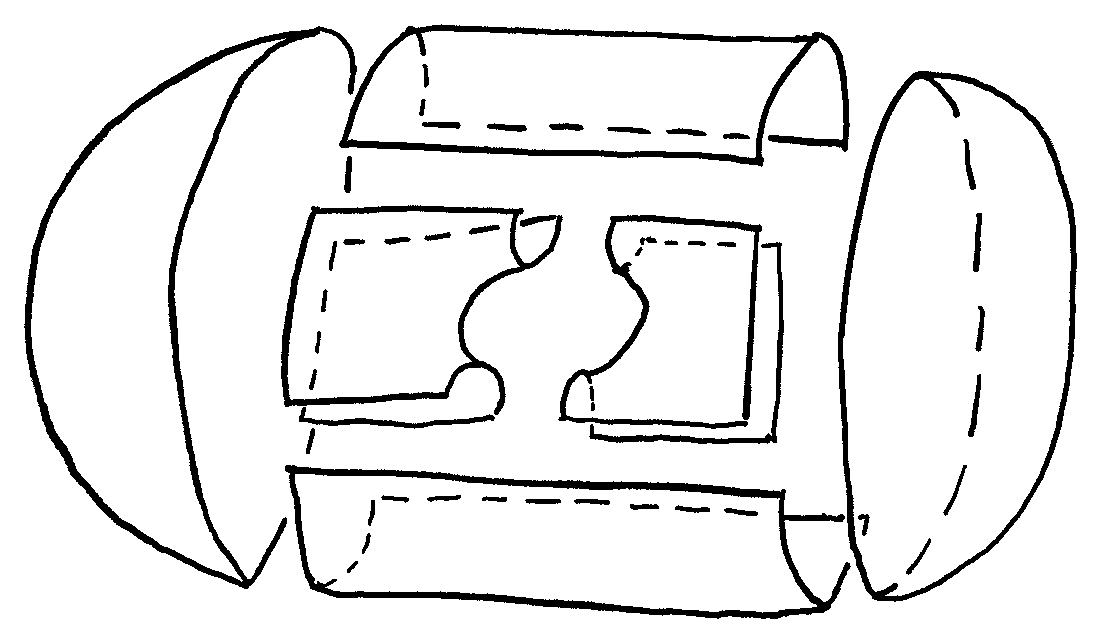
\includegraphics[width=9cm]{images/Final Lecture/TorusExtendedCut.png} 
        \caption{\small{Visualization of a torus extended down to a point. The vertices of the corners of the 2-dimensional surfaces are points.}}
        \label{CUTTORUS}
    \end{figure}
    
    Treating a TFT as a symmetric monoidal weak 2-functor (see \ref{Weak2Fun} for a definition)
     from
     a symmetric monoidal bicategory 
    $\Bord_{n,n-1,n-2}$
    (see \ref{SymmMonBicategory} for a definition), instead of from a symmetric monoidal category
     is
     named 'once-extended TFT', e.g. see \cite{SchwHopfQuantumTFT}. There are two important
      results
      regarding once-extended TFTs: 
    \begin{enumerate}
\item One regards the classification of 2d-TFTs down to a point and is due to Christopher Schommer Pries who
 proved it in his PhD thesis 
 $$
 ev_{\ast}:
 \Fun^\otimes (\Bord_{2,1,0}^{\fr}, \bat) \xrightarrow{\simeq} (\bat^{2\operatorname{-dualizable}})^{\cong} $$
\item The other, although still conjectural\footnote{It was first stated by Kevin Walker and then some progress was made by Turaev, see \cite{Turaev+2016} for more on this.}, classifies 3d-TFTs via the evaluation on the circle
$$  ev_{S^1}:\Fun^\otimes (\Bord_{3,2,1}^{\fr}, \operatorname{ModTensor}) \xrightarrow{\simeq}(\operatorname{ModTensor}^{2\operatorname{-dualizable}})^{\cong}$$ %unsure about the statement, did not find clearr references /ANdrea
hence $\Zf(S^1)=\cat$ where $\cat$ is a modular tensor category, i.e. a special ribbon category which can be seen as a categorified commutative Frobenius algebra.
    \end{enumerate}
    
    However, as one can infer from the aforementioned cobordism hypothesis, one can also extend downward to dimension $0$ any $n$-dimensional TFT and it was first proposed by Daniel Freed in \cite{Freed_1994}. To be precise, one nowadays does not want to only extend 
    downwards but also upwards, i.e. to not work wirh $n$-categories, i.e. $(n,n)$-categories,
     but wants to work with$(\infty,n)$-categories, i.e. categories where morphisms of dimension
      strictly greater than $n$ are invertible, because of technical reasons\footnote{For example, the
         argument sketched in \cite{lurie2009classification} is crucially a proof by induction on $n$
          and in order to understand the $n+1$-morphisms of $\Bord_{n+1}$ one must understand
           such $n+1$-morphisms in $\Bord_{n}$ which are absent if we treat $\Bord_{n}$ as an
            $n$-category and not $(\infty,n)$-category. In short, that would just not be possible
             without such $\infty$-categorical machinery.}. 
     Sketchily, the $(\infty,n)$ category of bordisms will have points as objects, bordisms between
      points as 1-morphisms, bordisms between bordisms between points as 2-morphisms,...,
       bordisms between bordisms between bordisms...\footnote{There is exactly $n-1$ times
         'between bordisms' after the first instance of 'bordisms', $n$-morphisms are morphisms
          between $(n-1)$-morphisms.} as $n$-morphisms, diffeomorphisms between
           $n$-dimensional bordisms as $n+1$-morphisms, isotopies between diffeomorphisms as
            $n+2$-morphisms, isotopies between isotopies between diffeomorphsims as
             $n+3$-morphisms, ... and so on infinitely many times.
              This is an example of a $(\infty,n)$-category, since isotopies of diffeomorphisms and
               diffeomorphisms are in fact invertible, whereas oriented bordisms not necessarily.
                One can find more on this higher category of bordisms in \cite{Calaque_2019}. 

\end{rem}

\subsection{Alternative formulation of the cobordism hypothesis of TFTs \extra}\label{FREEBORD}

It is not evident why the classification of extended TFTs by dualizable objects in the target category
goes by the name 'cobordism hypothesis'. The reason is that historically (in \cite{Baez_1995}) it was not
only formulated
 as the equivalence categories
 $$ev_{\ast}:\Fun^{\otimes}(\Bord_{n}^{\fr},\cat)\simeq (\cat^{\operatorname{fd}})^{\cong}$$
 but also in an equivalent way that is a vast generalization of the fact that $\Omega_{0}^{\operatorname{or}}$ is the free
  abelian group on one generator, i.e. $\Z$. 
  \begin{thm}[Cobordism Hypothesis]
$\Bord_{n}^{\fr}$ is equivalent to the free symmetric monoidal $(\infty,n)$-category with duals on one object.
  \end{thm}
  This is equivalent to the usual formulation via abstract nonsense. We first show how this works
   for the cobordism hypothesis
  in one dimension, which coincides with the classification we already proved, \ref{ClassificationOf1dTFTs}.
  \subsubsection{Categorification of  \texorpdfstring{$\Omega_{0}^{\operatorname{or}}=\Z$}{0}}\label{FREEBORD1}
  We already told a story about TFTs being a categorification of bordism invariants, see \ref{ClassificationOfTFTs}.
  This story fits very well with the cobordism hypothesis in dimension 1 and the fact that 
  $\Omega_{0}^{\operatorname{or}}$ is the free abelian group on one generator. 
  
  The cobordism hypothesis
  can be formulated in dimension 1 as follows 
  \begin{thm}[Cobordism hypothesis for $n=1$]
$\Bord_{1,0}^{\fr}$ is equivalent to the free symmetric monoidal category with duals on one object. More precisely,
$\Bord_{1,0}^{\fr}$ is equivalent to the image of the free functor $DFree:\Cat\to\operatorname{SymmMonwDuals}$
on the trivial category $\unit_{\Cat}$, where SymmMonwDuals denotes the category of symmetric monoidal categories
with duals. 
$$\Bord_{1,0}^{\fr}\simeq DFree(\unit_{\Cat})$$
  \end{thm}
This is equivalent to the classification of 1TFTs, the theorem we proved stating that 
\begin{thm}[Classification of 1TFTs]
$$ev_{\ast}:\Fun^{\otimes}(\Bord_{1}^{\operatorname{or}},\cat)\simeq (\cat^{\operatorname{fd}})^{\cong}$$
\end{thm}
 
 First, note that there are no non-trivial tangent bundles on 1-bordisms and thus there is no difference between 
 framed and oriented bordisms. Thus, one can infer from the classification of 1TFTs a version of the cobordism 
 hypothesis in dimension $n=1$ as we first stated it:
 $$ev_{\ast}:\Fun^{\otimes}(\Bord_{1}^{\operatorname{fr}},\cat)\simeq (\cat^{\operatorname{fd}})^{\cong}$$
  Then, we make precise what is a free symmetric monoidal category with duals on one object.
\begin{notat}
We denote as SymmMonwDuals the category of symmetric monoidal categories with dual objects.
\end{notat}
Now we prove the following theorem in three steps
\begin{thm}
	For a symmetric monoidal category with duals $\cat$ it holds that
	$$\Fun^{\otimes}(\Bord_{1,0}^{\operatorname{or}},\cat)\overset{1}{\simeq}\Fun^{\otimes}(DFree(\unit_{\Cat}),\cat^{\cong})\overset{2}{\simeq}\Fun(\unit_{\Cat},DForget(\cat^{\cong}))\overset{3}{\simeq} \cat^{\cong}$$
\end{thm}
\begin{proof}
	%Note first that for any three symmetric monoidal categories $\sat$, $\dat$ and $\eat$ it holds that if $\dat\simeq\eat$, then
%	$\Fun^{\otimes}(\dat,\sat)\simeq\Fun^{\otimes}(\eat,\sat)$. MIght be false
\begin{enumerate}
\item Consider the forgetful functor $DForget:\operatorname{SymmMonwDuals}\to\Cat$. 
 Like all forgetful functors it has 
a left adjoint $DFree:\Cat\to\operatorname{SymmMonwDuals}$.
The application of this functor to the trivial category\footnote{i.e. the category just with one-object and its
	identity morphism.} $\unit_{\Cat}$ is the free symmetric monoidal category on one object.

From the proofs \ref{abstractClass1TFT} and \ref{GeneratorsClass1TFT} of the classification of 1TFTs
one can easily infer that $\Bord_{1}^{\fr}$ is equivalent to the free symmetric monoidal category with duals
on one object,
$\Bord_{1}^{\fr}\simeq DFree(\unit_{\Cat})$
and thereby proving the alternative formulation of the cobordism hypothesis in dimension 1 we just provided. Moreover,
reacall that $\Fun^{\otimes}(\Bord_{1,0}^{\operatorname{or}},\cat)$ is a groupoid and hence
the functor
$$\Fun^{\otimes}(\Bord_{1,0}^{\operatorname{or}},\cat)\to\Fun^{\otimes}(DFree(\unit_{\Cat}),\cat)$$
can be restricted to the equivalence
 $$\Fun^{\otimes}(\Bord_{1,0}^{\operatorname{or}},\cat)\overset{1}{\simeq}\Fun^{\otimes}(DFree(\unit_{\Cat}),\cat^{\cong})$$

\item Note that there is another way to phrase adjunctions, which we formulated in the appendix, \ref{HigherAdjFun}, and
also that the functor in SymmMonwDuals are just symmetric monoidal functors, since functors preserve dual
objects, as we proved in \ref{ClassificationOf1dTFTs}.
From the free-forgetful adjunction, one can infer that for an arbitrary symmetric monoidal category with duals $\cat$
$$\Fun^\otimes (DFree(\unit_{\Cat}),\cat^{\cong})\overset{2}{\simeq}\Fun(\unit_{\Cat},\cat^{\cong})$$
where on the right hand side $\cat$ has forgotten about its duals and its monoidal structure generally. 


\item Now we prove that $\Fun(\unit_{\Cat},DForget(\cat^{\cong}))\overset{3}{\simeq} \cat^{\cong}$.
$\Fun(\unit_{\Cat},\cat)$ consists of functors $$F(\ast)=X$$ $$F(id_\ast)=id_X$$ for all $X\in\cat$
The morphisms of $\Fun(\unit_{\Cat},\cat)$ are exactly given by the morphisms in $\cat$:  given two functors
 $F,G\in\Fun(\unit_{\Cat},\cat)$ such that $F(\ast)=X$ and $G(\ast)=Y$,
 there is a natural transformation $F\Rightarrow G$, if and only if
there is a morphism $f:X\to Y$ in $\cat^{\cong}$ because so the square 
% https://q.uiver.app/#q=WzAsNCxbMCwwLCJcXGFzdCJdLFswLDEsIlxcYXN0Il0sWzEsMCwiWCJdLFsxLDEsIlkiXSxbMCwxLCJpZF9cXGFzdCIsMl0sWzAsMiwiRiJdLFsxLDMsIkciLDJdLFsyLDMsImYiXV0=
\[\begin{tikzcd}[cramped]
	\ast & X \\
	\ast & Y
	\arrow["{id_\ast}"', from=1-1, to=2-1]
	\arrow["F", from=1-1, to=1-2]
	\arrow["G"', from=2-1, to=2-2]
	\arrow["f", from=1-2, to=2-2]
\end{tikzcd}\]
commutes. Clearly the functor $\Fun(\unit_{\Cat},DForget(\cat^{\cong})\to \cat^{\cong}$ is essentially surjective
since for every object $X\in\cat^{\cong}$ there is a functor $F\in\Fun(\unit_{\Cat},DForget(\cat^{\cong})$ such that
$F(\ast)=X$. Moreover, since any natural transformation in $\Fun(\unit_{\Cat},DForget(\cat^{\cong})$ is given by
a morphism in $\cat^{\cong}$, $\Fun(\unit_{\Cat},DForget(\cat^{\cong})\to \cat^{\cong}$ is fully faithful.
Thus, we can conclude that 
$$\Fun(\unit_{\Cat},DForget(\cat^{\cong}))\overset{3}{\simeq} \cat^{\cong}$$
\end{enumerate}
\end{proof}

\begin{rem}
The assumption that $\cat$ has duals does not imply a loss of generality 
since the functor 
$$\Fun^{\otimes}(\Bord_{1,0}^{\operatorname{or}},\cat^{\fd})\to\Fun^{\otimes}(\Bord_{1,0}^{\operatorname{or}},\cat)$$
is canonically an equivalence since $\Bord_{1,0}^{\operatorname{or}}$ has duals and always lands in
$\cat^{\fd}$
\end{rem}


Thus, one can infer the usual formulation as an equivalence by the
transitivity of equivalences of categories (a composition of equivalences is an equivalence), from the fact that $\Bord_{1,0}$ is the free
symmetric monoidal category with duals and 
 abstract nonsense.